\documentclass[a4paper, 11pt]{article}
\usepackage[utf8]{inputenc}
\usepackage{mathtools}
\usepackage{amsmath}
\usepackage{titlesec}
\usepackage{amssymb}
\usepackage{gensymb}
\usepackage[english]{babel}
\usepackage[dvipsnames]{xcolor}
\usepackage[margin=1in]{geometry}
\usepackage[hidelinks]{hyperref}
\usepackage{fancyhdr}
\usepackage{graphicx}
\usepackage{cancel}
\usepackage{float}
\usepackage{subcaption}
\usepackage{tabto}
\usepackage{tocloft}
\usepackage{xcolor}
\usepackage{yfonts}
\usepackage[style=numeric-comp, sorting=none]{biblatex}
\bibliography{bib.bib}
\newcommand{\figuretag}[1]{%
  \addtocounter{figure}{-1}%
  \renewcommand{\thefigure}{#1}%
}

\setcounter{tocdepth}{1}
\renewcommand{\cftdot}{.}

% Configurar las cabeceras para todas las páginas
\pagestyle{fancy}
\lhead{Entrega 1}
\rhead{}

% Para que la cabecera aparezca también en la primera página
\fancypagestyle{plain}{%
  \fancyhf{} % Limpiar cabeceras y pies de página
  \lhead{Entrega 1} % Añadir la cabecera en la primera página
  \rhead{} % Vaciar la cabecera derecha
}

\title{{\textbf{\Large ENTREGA 1: DIFRACCIÓ
}\\}}

\author{Reina Delgado, Airan (1670808)\\}

\date{}

\begin{document}

\maketitle

%%%%%%%%%%%%%%%%%%%%%%%%%%%%%%%%%%%%%%%%%%%%%%%%%%%%%%%%
%%%%%%%%%%%%%%%%%%%%%%%%%%%%%%%%%%%%%%%%%%%%%%%%%%%%%%%%
%%%%%%%%%%%%%%%%%%%%%%%%%%%%%%%%%%%%%%%%%%%%%%%%%%%%%%%%
%%%%%%%%%%%%%%%%%%%%%%%%%%%%%%%%%%%%%%%%%%%%%%%%%%%%%%%%
%%%%%%%%%%%%%%%%%%%%%%%%%%%%%%%%%%%%%%%%%%%%%%%%%%%%%%%%

\noindent \textcolor{red}{\textbf{Nota:} El codi emprat per a l'anàlisi de dades, els cálculs i la generació de grafics es pot trobar en el GitHub associat a aquesta entrega: \url{https://github.com/AiranReina/Estat_Solid}. El repositori serà emprat per a futures entregues, per tant, cal llegir el README per entendre l'estructura del mateix.}

\vspace{5mm}

\noindent Aquesta entrega tracta sobre l'anàlisi de dades obtingudes a partir d'un patró de difracció de raigs X ($\lambda = 1.5406 \text{\AA}$) d'un material cristal·lí d'estructura desconeguda. Els objectius són determinar quina estructura ajusta millor les dades experimentals i trobar la constant de xarxa $a$ del material. \textbf{En aquest document s'analitzen els resultats del fitxer CSV 19}. En la figura \ref{fig:patro} es mostra el patró de difracció obtingut.

\begin{figure}[h!]
    \centering
    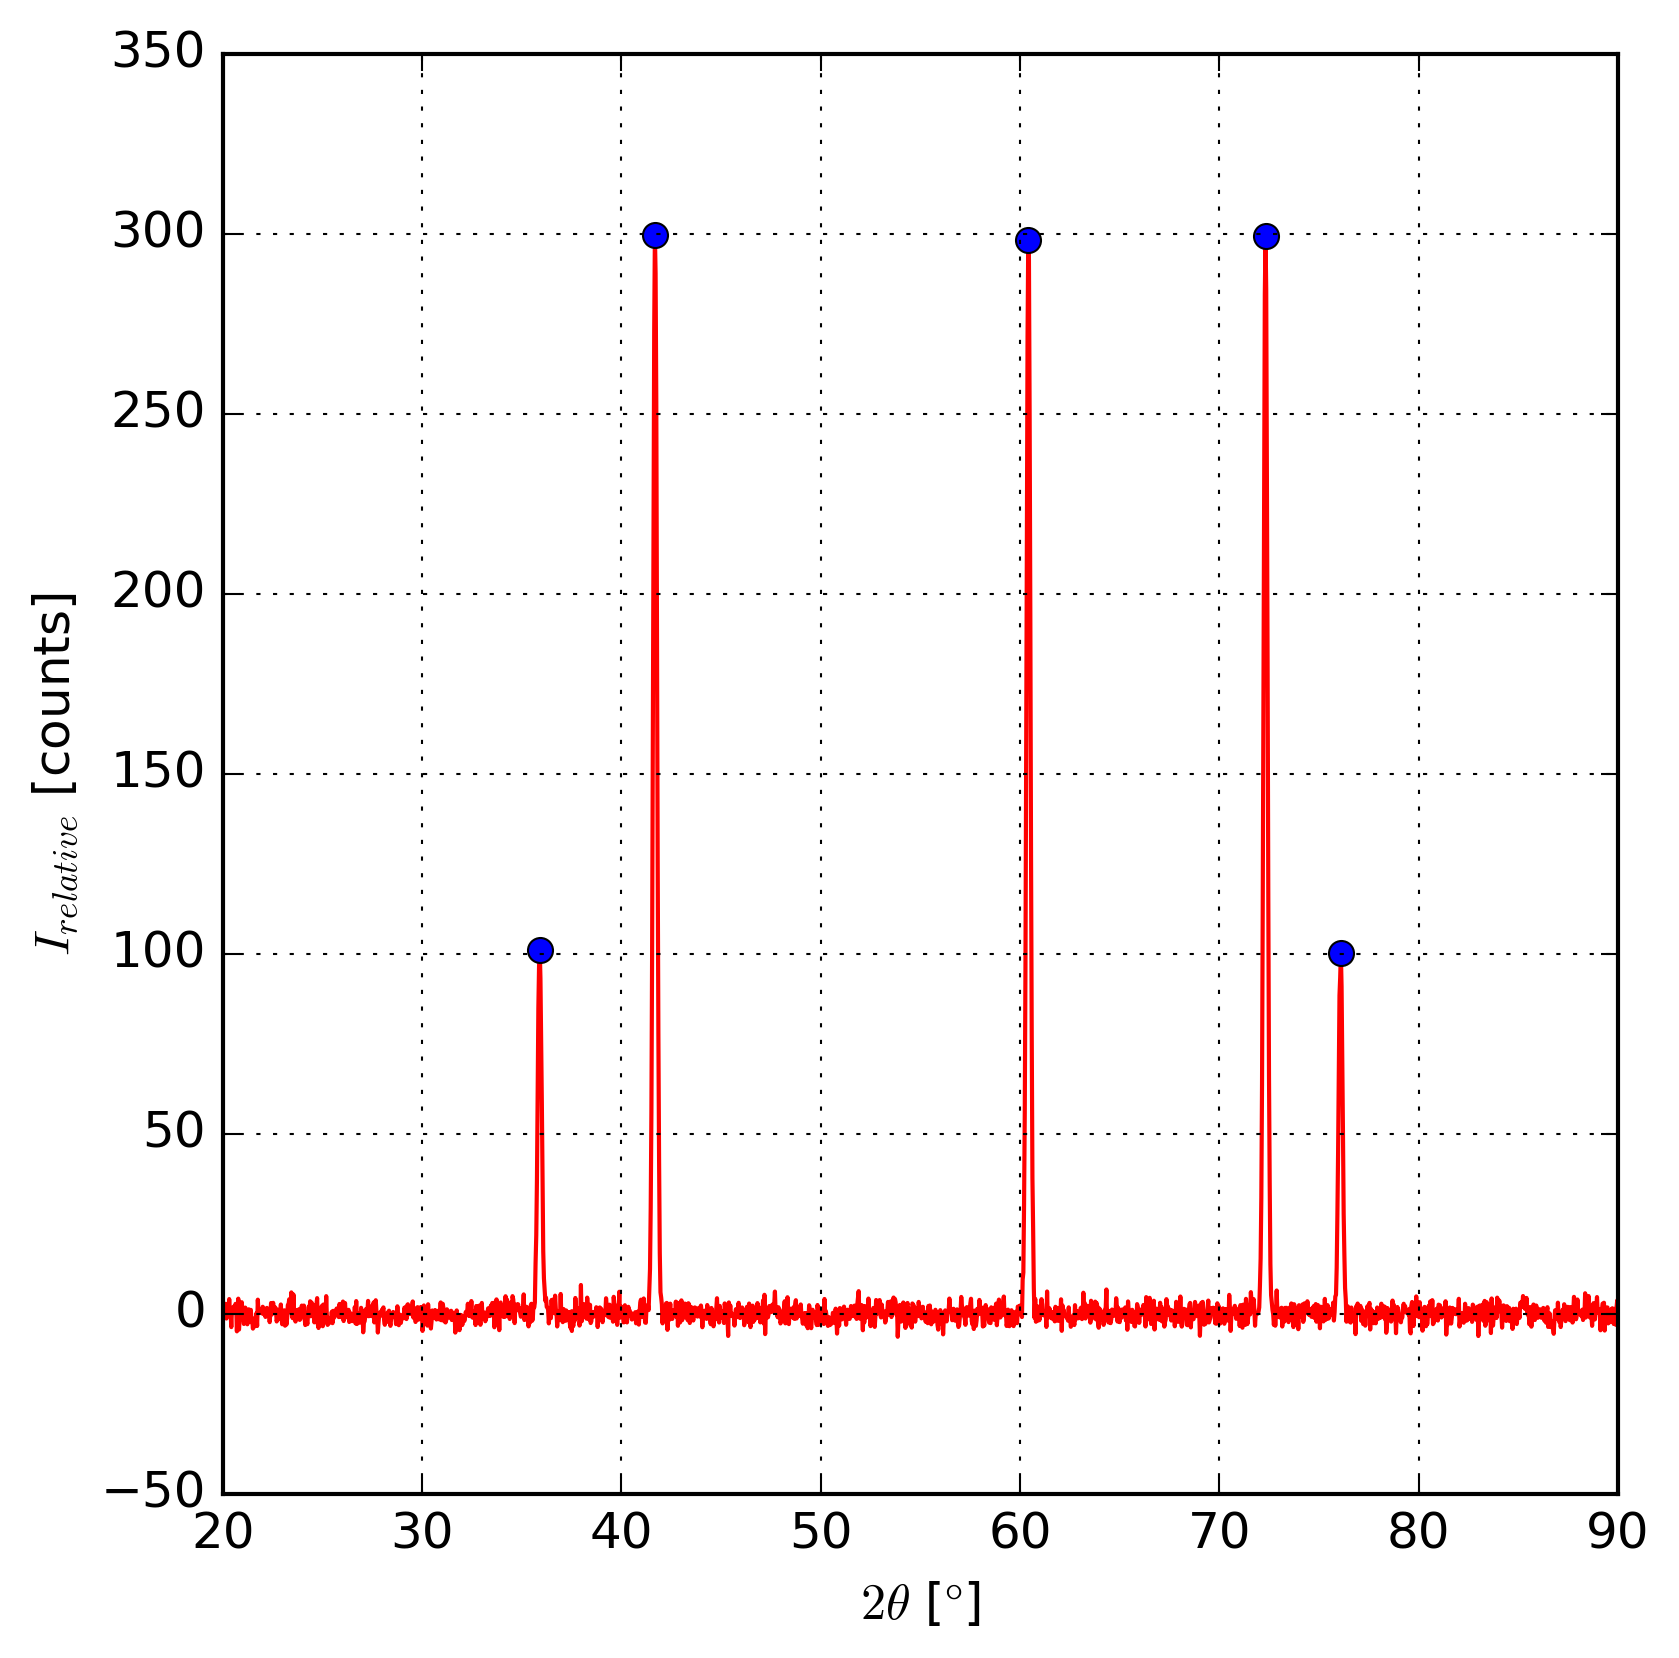
\includegraphics[width=0.7\textwidth]{images/grafic_experimental_peaks.png}
    \caption{Patró de difracció de raigs X obtingut experimentalment.}
    \label{fig:patro}
\end{figure}

\noindent Per realitzar l'anàlisi, s'ha emprat la funció "\textit{find\_peaks}" de la llibreria "\textit{scipy.signal}" per identificar els pics en el patró de difracció. Aquesta funció permet detectar els màxims locals en una sèrie de dades, facilitant la identificació dels angles de difracció corresponents als diferents plans cristal·lins. Per comprovar la veracitat dels pics de forma qualitativa, s'han representat sobre el patró de difracció, com es pot observar. Emprant aquets valors, podem convertir els angles de difracció $\theta$ en les separacions entre plans $d$ mitjançant la llei de Bragg:

\begin{equation}
    2d\sin(\theta) = m\lambda
\end{equation}

\noindent Ón $n$ és l'ordre de difracció (en aquest cas, $m=1$). Els valors tractats en aquesta discussió es poden trobar a la taula \ref{tab:valors}.

\begin{table}[h!]
    \centering
    \begin{tabular}{|c|c|c|}
        \hline
        Pic & $\theta$ (º) & $d$ (\AA) \\
        \hline
        1 & 17.95 & 2.50 \\
        2 & 20.84 & 2.17 \\
        3 & 30.21 & 1.53 \\
        4 & 36.16 & 1.31 \\
        5 & 38.05 & 1.25 \\
        \hline
    \end{tabular}
    \caption{Magnituds rellevants extretes experimentalment.}
    \label{tab:valors}
\end{table}

\noindent A continuació, es calcula el factor $1/d^2$ per a cada pic, ja que aquest és el que ajusta les diferents estructures cristal·lines considerades. Això es deu a que la relació entre $1/d^2$ i el modul al quadrat del vector recíproc generic $|\vec{G}|^2 \propto h^2 + k^2 + l^2$ d'una xarxa cúbica és lineal, on $h$, $k$ i $l$ són els índexs dels plans cristal·lins de difracció. Si l'estructura és cúbica simple (SC), s'observarien pics en tots els valors de $h$, $k$ i $l$ (Obviant, obviament, les combinacions $(h,k,l)$ que generen plans que disten el mateix), mentre que per a les altres estructures (Considerarem cúbica centrada en el cos (BCC), cúbica centrada en les cares (FCC) i diamant) només es permeten certes combinacions d'índexs ja que l'adició d'àtoms en posicions específiques dins de la cel·la unitària provoca interferències destructives que cancel·len alguns pics de difracció. La relació esmentada és la següent:

\begin{equation}
    \frac{1}{d^2} = \frac{h^2 + k^2 + l^2}{a^2}
    \label{eq:relacio}
\end{equation}

\noindent És important observar que la constant de proporcionalitat depén de la constant de xarxa $a$ tal que $a = 1/\sqrt{\text{pendent}}$. Per demostrar la relació \ref{eq:relacio}, començem per la definició del vector recíproc $\vec{G}$, que diu $\vec{G} · \vec{T} = 2\pi m$, ón $\vec{T}$ és un vector de la xarxa directa i $m$ és un enter. Si ens centrem en un àtom en $\vec{T_0}$, l'àtom en el pla següent segueix l'expressió $\vec{G} · (\vec{T_0} + d\hat{n}) = 2\pi (m+1)$. Si restem ambdues expressions, obtenim que $\vec{G} · d\hat{n} = |\vec{G}|d= 2\pi$ i, si elevem al quadrat i aïllem $1/d^2$, obtenim $\frac{1}{d^2} = \frac{|\vec{G}|^2}{(2\pi)^2}$. Si estudiem una cel·la cúbica, podem expressar el vector recíproc com $\vec{G} = \frac{2\pi}{a}(h,k,l)$. Si fiquem aquest valor a l'expressió anterior, obtenim la relació \ref{eq:relacio}.

\vspace{5mm}

\noindent Amb aquests resultats, podem seguir el seguent procediment per determinar l'estructura cristal·lina i la constant de xarxa $a$ del material: Utilitzant el factor d'estructura, estudiem quan aquest dona interferències destructives per cada estructura cristal·lina; els valors $(h,k,l)$ que anulen el factor d'estructura són eliminats de la llista de possibles valors per cada estructura; a continuació grafiquem $1/d^2$ en funció de $h^2 + k^2 + l^2$ per als valors restants (Com observem 5 pics, utilitzarem els primers 5 valors de $h^2 + k^2 + l^2$ que compleixin les condicions de cada estructura); finalment, realitzarem un ajust lineal, aquell amb millor coeficient de correlació serà l'estructura cristal·lina del material i la pendent ens permetrà calcular la constant de xarxa $a$. Les regressions de les estructures proposades es poden observar a la figura \ref{fig:grafics}.

\vspace{5mm}

\begin{figure}[htbp]
  \centering

  \begin{subfigure}[b]{0.48\textwidth}
    \centering
    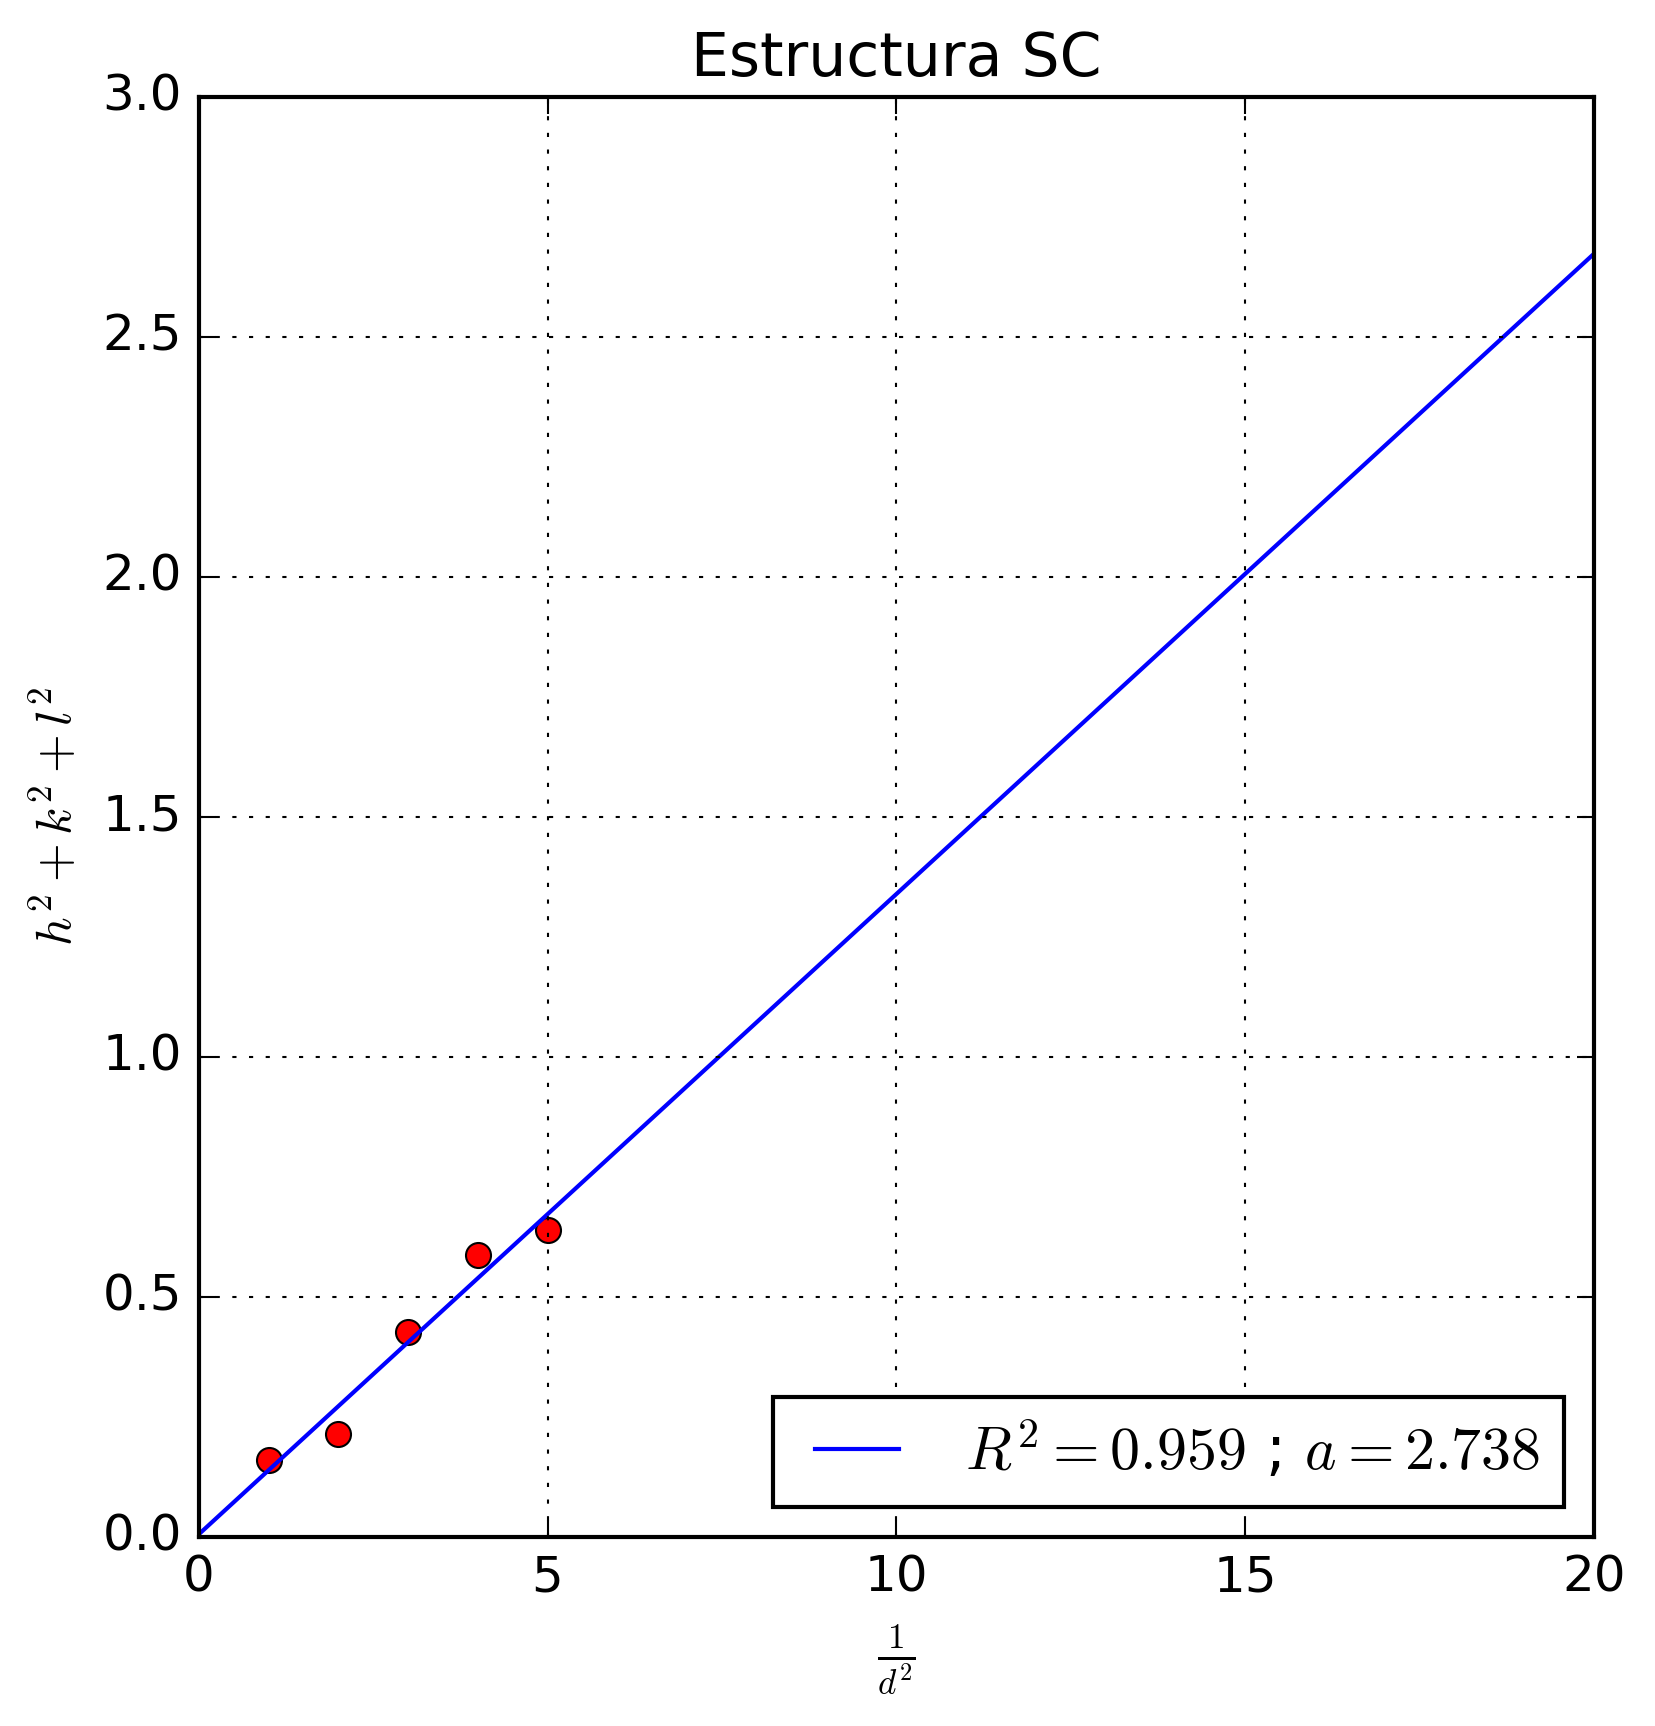
\includegraphics[width=\linewidth]{images/SC.png}
    \caption{Estructura cúbica simple (SC)}
    \label{fig:1}
  \end{subfigure}
  \hfill
  \begin{subfigure}[b]{0.48\textwidth}
    \centering
    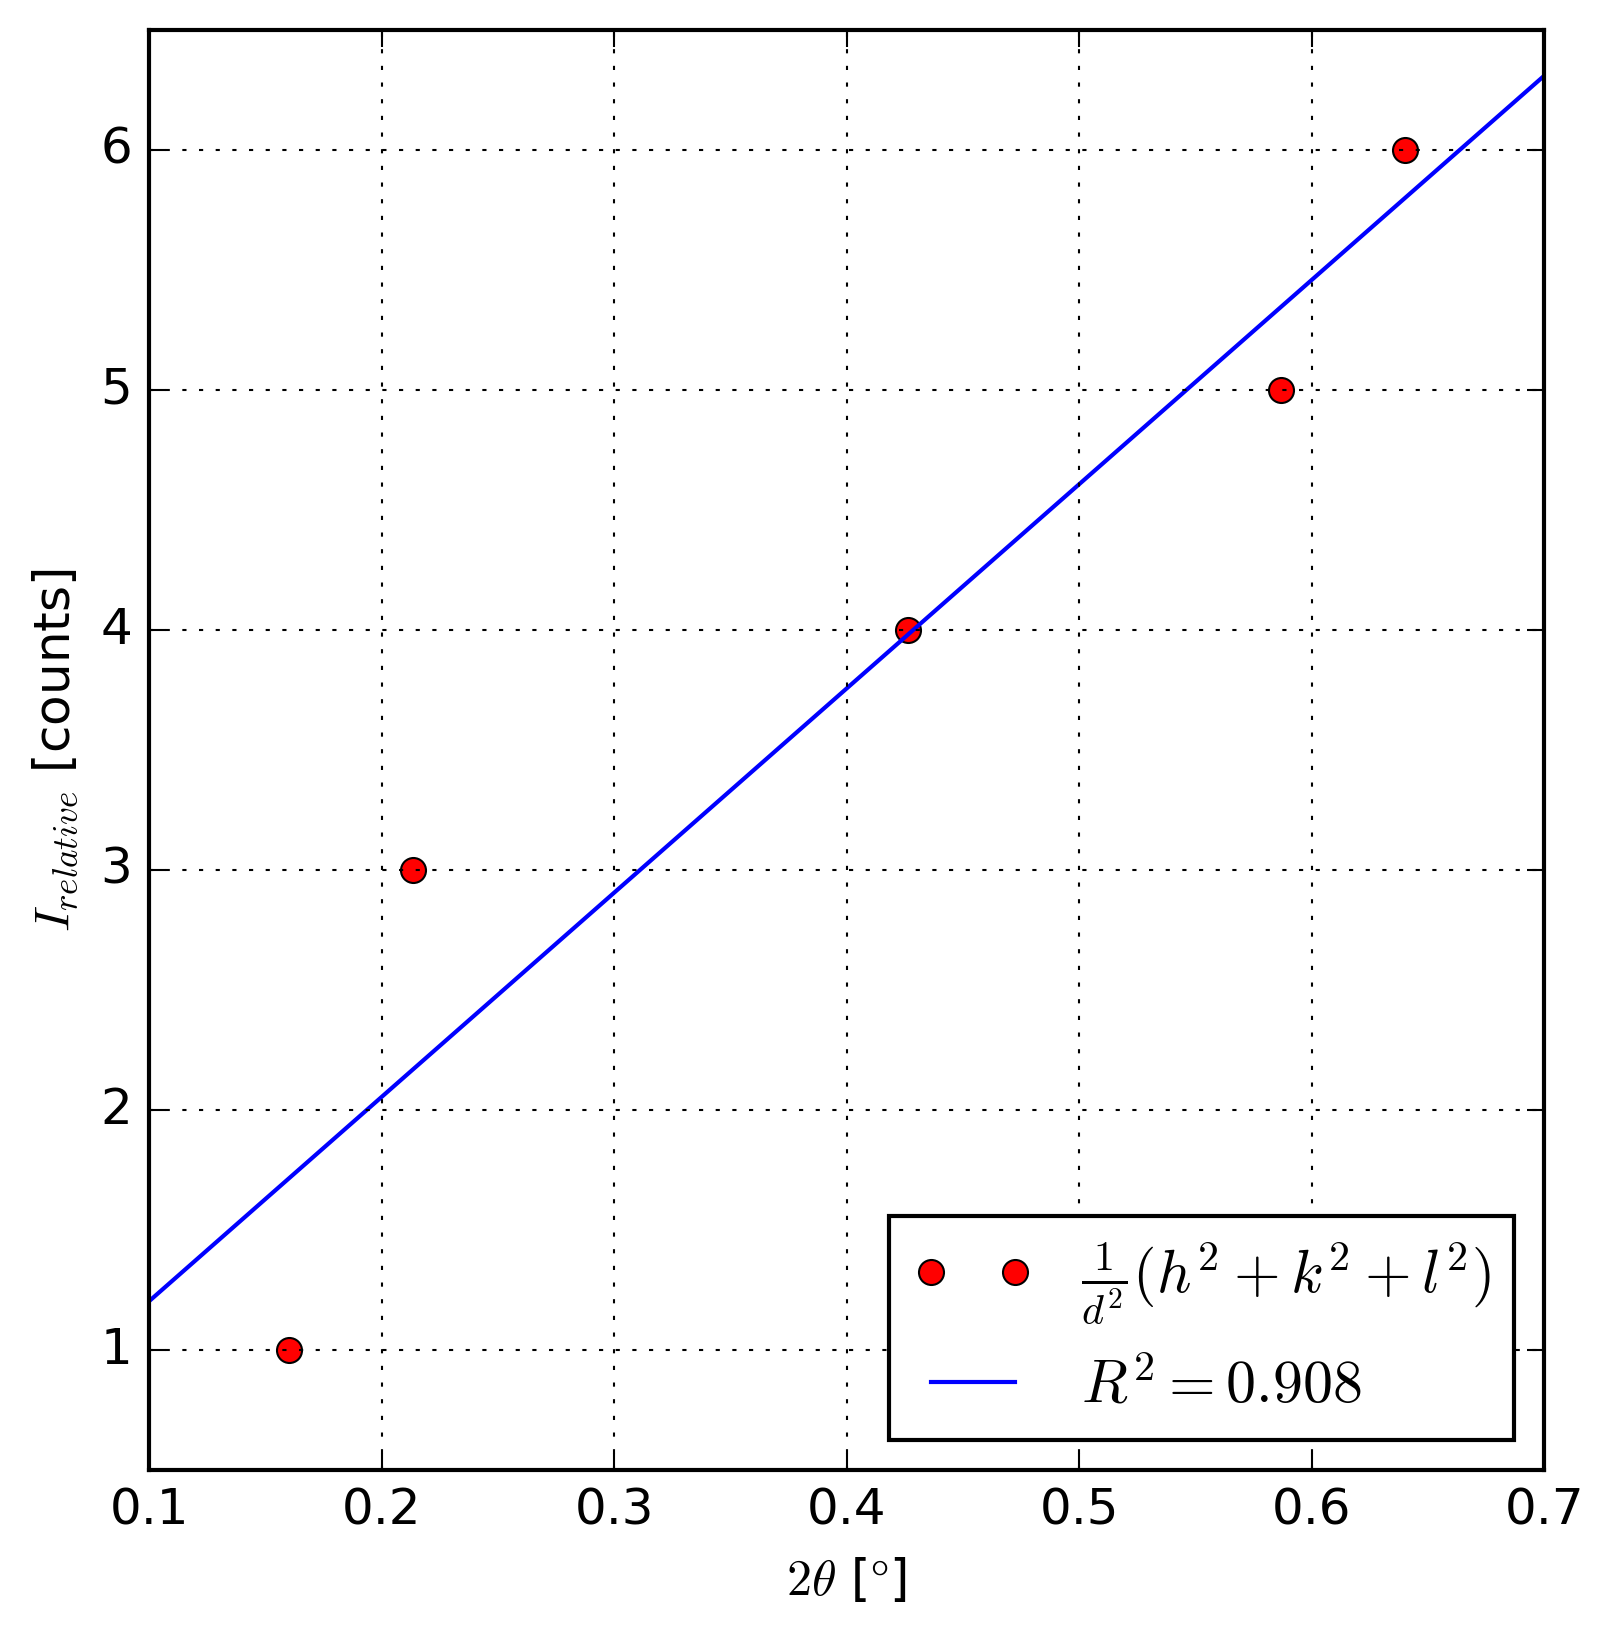
\includegraphics[width=\linewidth]{images/FCC.png}
    \caption{Estructura cúbica centrada en les cares (FCC)}
    \label{fig:2}
  \end{subfigure}

  \vspace{0.5em}


  \begin{subfigure}[b]{0.48\textwidth}
    \centering
    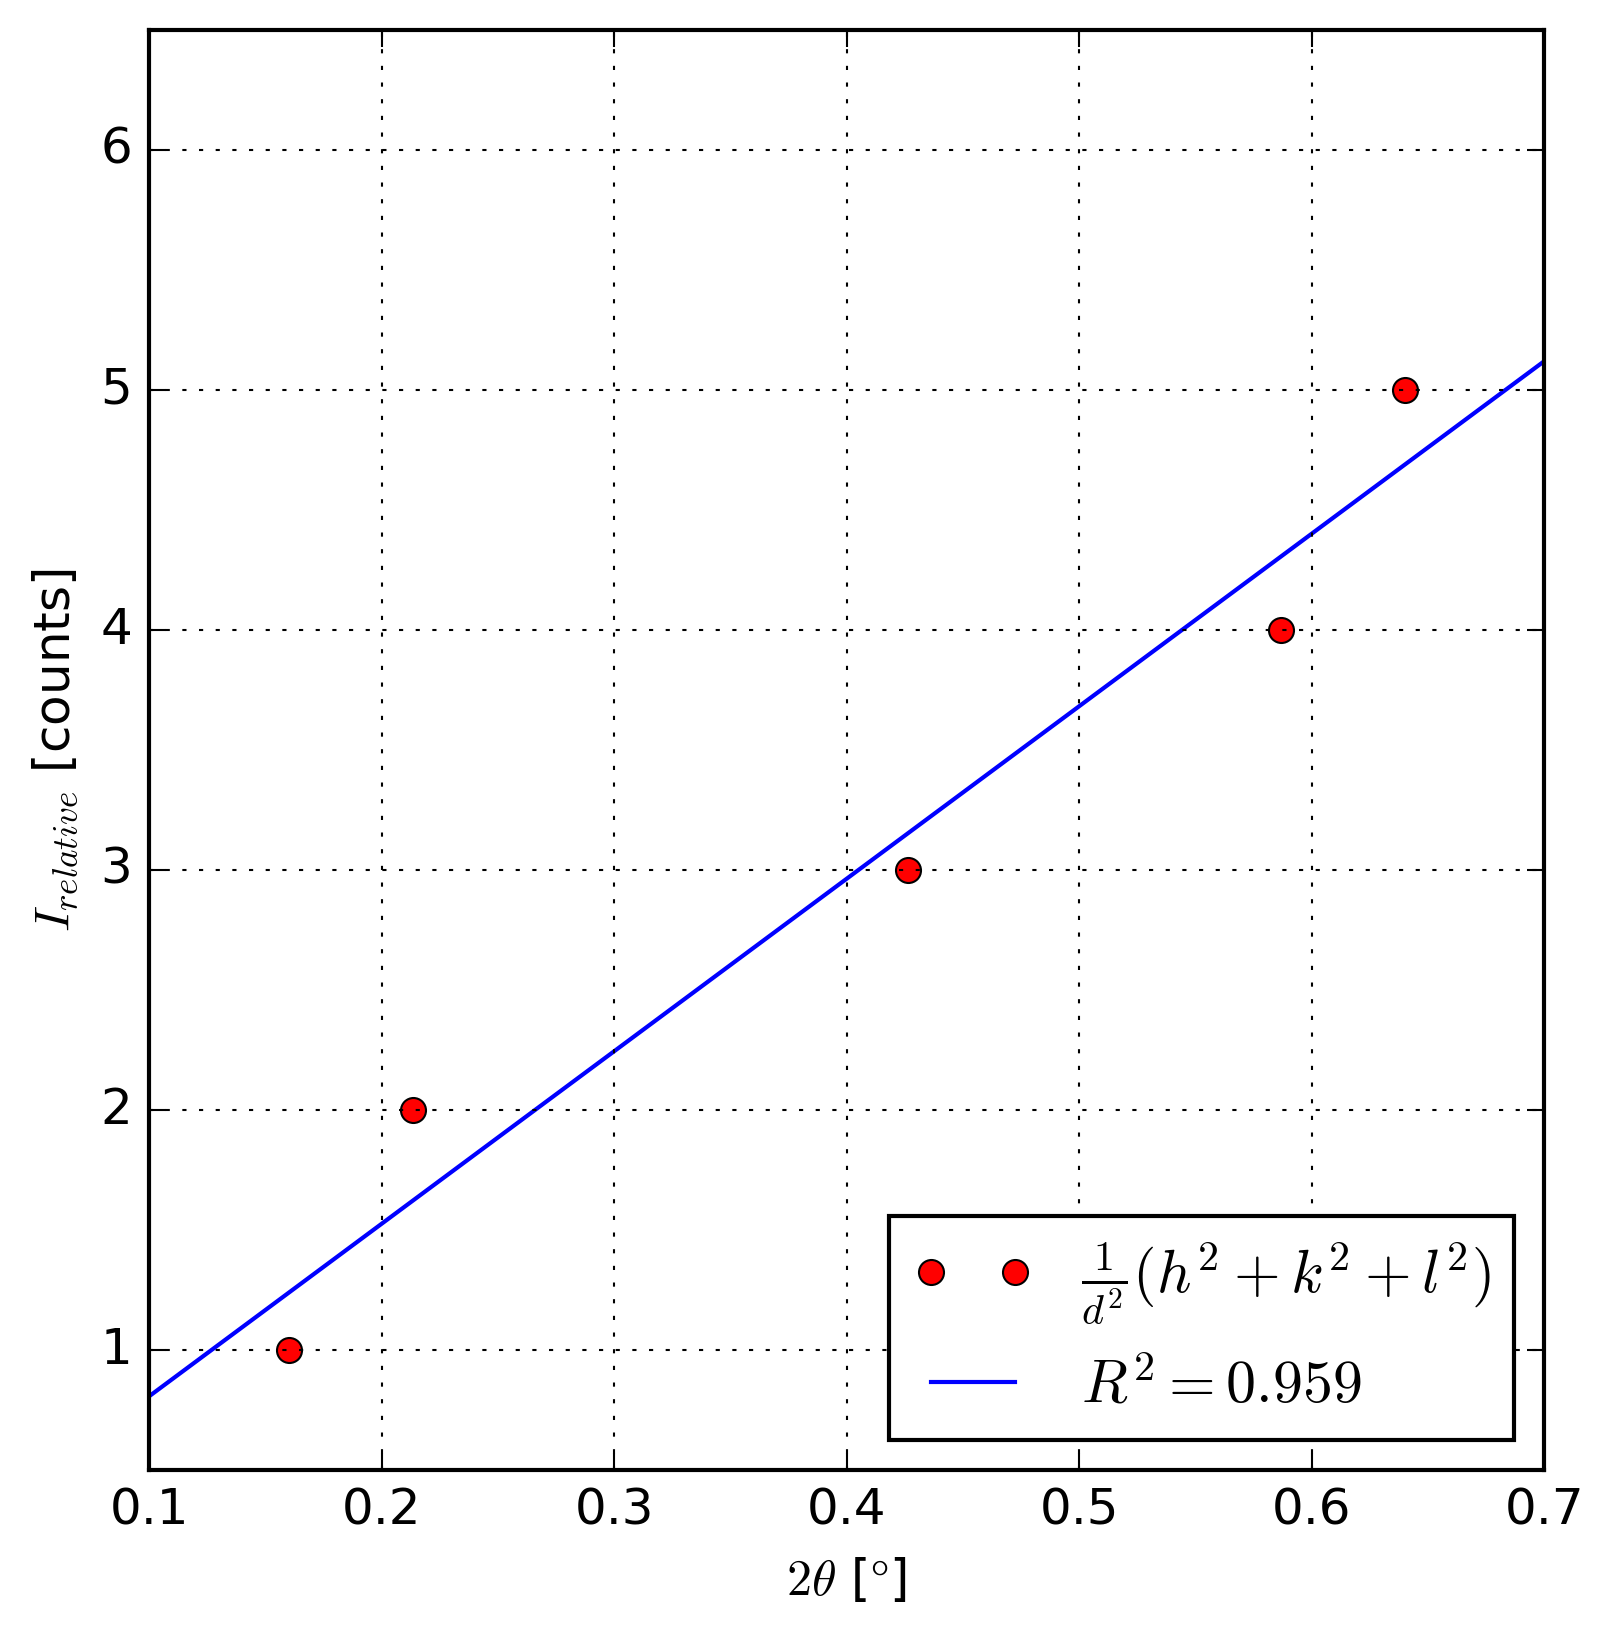
\includegraphics[width=\linewidth]{images/BCC.png}
    \caption{Estructura cúbica centrada en el cos (BCC)}
    \label{fig:3}
  \end{subfigure}
  \hfill
  \begin{subfigure}[b]{0.48\textwidth}
    \centering
    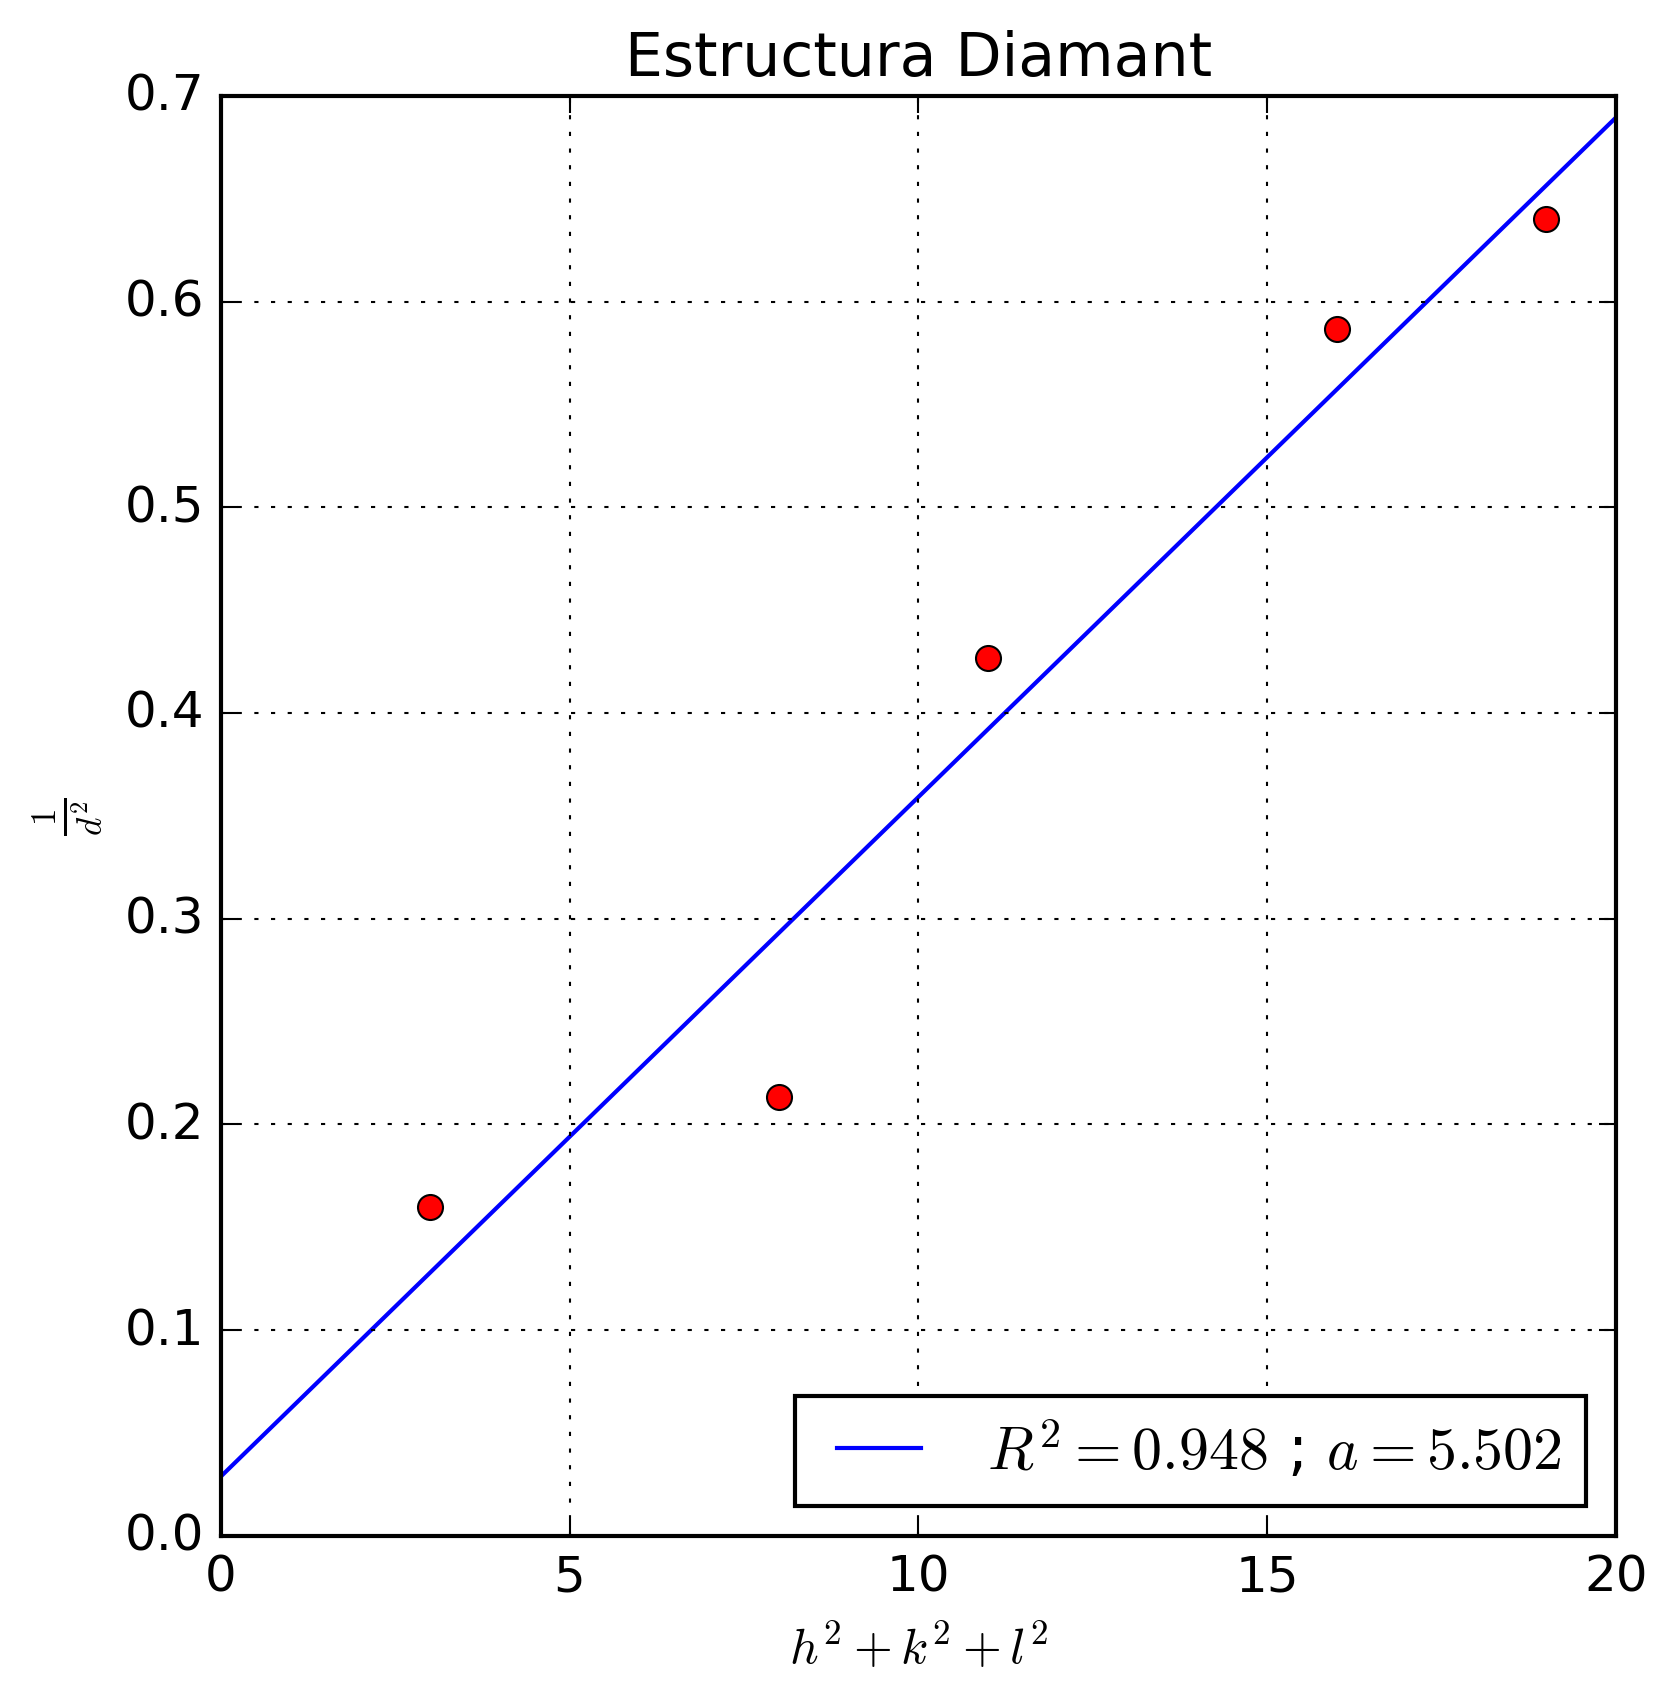
\includegraphics[width=\linewidth]{images/Diamant.png}
    \caption{Estructura de diamant}
    \label{fig:4}
  \end{subfigure}

  \caption{Regressions lineals per a les diferents estructures cristal·lines considerades.}
  \label{fig:grafics}
\end{figure}

\noindent Observem que l'estructura que millor ajusta les dades és la cúbica centrada en les cares (FCC), ja que és l'única que aconsegueix un coeficient de correlació $R^2$ d'1 (En general és suficient amb emprar la que millor ajusta però, en aquest cas, és exacte). Com s'ha explicat anteriorment, la pendent de la recta ens permet calcular la constant de xarxa $a$ del material. En aquest cas, la constant de xarxa és $a = 1/\sqrt{pendent} = 4.33 \text{\AA}$.

%%%%%%%%%%%%%%%%%%%%%%%%%%%%%%%%%%%%%%%%%%%%%%%%%%%%%%%%
%%%%%%%%%%%%%%%%%%%%%%%%%%%%%%%%%%%%%%%%%%%%%%%%%%%%%%%%
%%%%%%%%%%%%%%%%%%%%%%%%%%%%%%%%%%%%%%%%%%%%%%%%%%%%%%%%
%%%%%%%%%%%%%%%%%%%%%%%%%%%%%%%%%%%%%%%%%%%%%%%%%%%%%%%%
%%%%%%%%%%%%%%%%%%%%%%%%%%%%%%%%%%%%%%%%%%%%%%%%%%%%%%%%

\end{document}